\chapter{Contextualization of the Learning Factory}

\section{Industry 4.0}
The Fourth Industrial Revolution (Industry 4.0) is considered a new industrial stage integrating the manufacturing environment with the cyber world to form cyber-physical systems (CPS) (\cite{jazdi2014}; \cite{wang2015}). This transition creates opportunities towards more autonomous and intelligent production lines (\cite{malburg2020}). To conduct research in this field without depending on expensive production lines, learning factories are used to physically model realistic shop floors on a smaller scale (\cite{malburg2020}). The thesis extensively uses the Fischertechnik learning factory when conducting research on refactoring. This allows to run experiments at low costs and transfer results to real smart factories (\cite{malburg2020}), a key construct of industry 4.0. (\cite{osterrieder2020}). 

Throughout this thesis, different terms are used to reference the case study. When referring to the hardware environment of the learning factory, the term CPS is used. For discussing the software elements of the learning factory, the term \emph{software system} is used. Further, when collectively concentrating on hardware and software, the term \emph{learning factory} or simply \emph{factory} is used.

\section{Industry demands of Refactoring}
Industry 4.0 is closely linked with the business space. Industry-wide developments promise more efficient production processes, optimized supply chains, and cost reductions \cite{malburg2020}. By the increasing relevance of software within the industry, implications on business when refactoring should also be taken into consideration. Section \ref{sec:business-case} explains the concept of technical debt, which provides a foundation to argue for refactoring from a business perspective. Further, once a business case for refactoring is established, industries want to efficiently allocate their resources. Section \ref{sec:economic-decisions} elaborates on the topic of justifying company-wide decisions on refactoring and discusses the communication of the decisions.

Moreover, by examining refactoring theory, businesses are able to learn the benefits of refactoring (see section \ref{sec:benefits}) and understand what criteria influence refactoring (see section \ref{sec:criteria}). In addition, to fully profit from refactoring, organizations should have an understanding of associated challenges (see section \ref{sec:challenges}) and challenges specific to CPS (see section \ref{sec:cps}).

\section{Fischertechnik Learning Factory}
\label{sec:fischertechnik}

\begin{figure}[H]
    \centering
    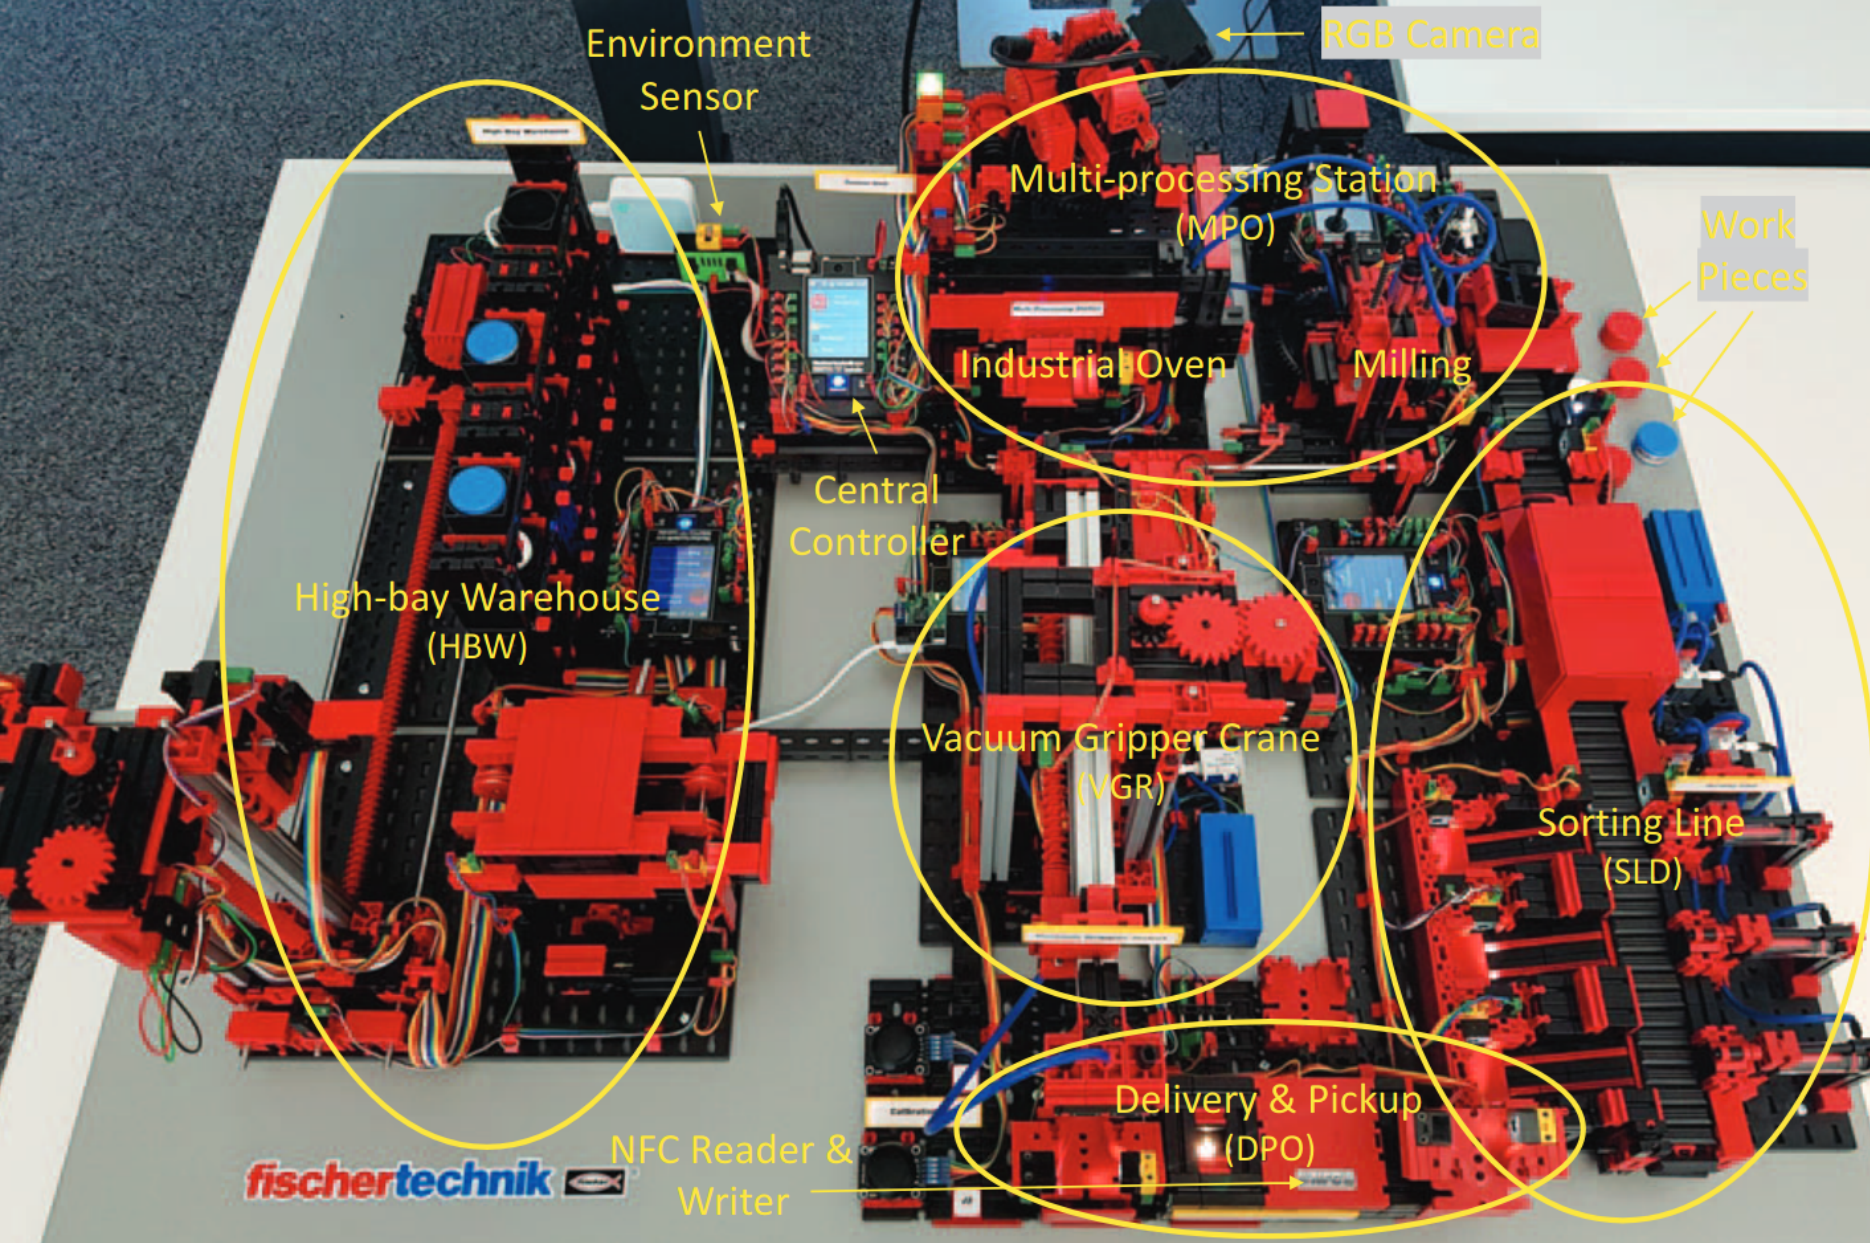
\includegraphics[width=\textwidth]{./assets/factory}
    \label{fig:factory}
    \caption{Fischertechnik Learning Factory (\cite{seiger2020})}
\end{figure}

% Hardware
Figure \ref{fig:factory} presents an overview of the learning factory utilized in the thesis. The factory consists of five workstations: a sorting line (SLD) with color detection, a multi-processing station (MPO), a milling machine (MM), a high-bay warehouse (HBW), and a vacuum gripper robot (VGR) (\cite{seiger2020}). Including sensors, actuators and the Fischertechnik TXT controllers, the learning factory features a complete production line (\cite{malburg2020}).

To enable programming of the learning factory on the abstraction level of business processes, \textcite{malburg2020} found that an additional software stack is required on top of the existing IoT components. The software system used for the case study, fully implemented this abstraction, by using web services. This enables the learning factory to be controlled by a process automation platform called \emph{Camunda} using Business Process Model and Notation (BMPN). 

However, the contribution of computer code that was needed to achieve this task has not been refactored. In addition, it is envisioned for the software system to migrate towards microservices. In particular, it would be desirable for each workstation to be its own microservice. For instance, fault tolerance could be introduced, by having the ability to restart each station independently.  These conditions inspire an exploration into refactoring this software system. Given the present circumstances of the learning factory, it is appropriate to analyze both the methods (see chapter \ref{chapter:methodology}) and the necessity (see chapter \ref{chapter:findings}) of refactoring this system. 